\documentclass[sigplan,review]{acmart}
\setcopyright{none}
\acmConference{PEPM}{2023}{Boston}

\usepackage{graphicx,color}
\usepackage{subcaption}
\usepackage{braket}
\usepackage{minted}
\usepackage{yquant}
\usepackage{multirow}
\usepackage{enumitem}
\usepackage{tikz}
\usetikzlibrary{quantikz,fit,quotes,svg.path}
%%\usepackage[backend=biber,citestyle=numeric-comp]{biblatex}
%%\ExecuteBibliographyOptions{sorting=nyt,maxbibnames=100,doi=false,isbn=false,url=false}
%%\addbibresource{cites.bib}
\bibliographystyle{acm}

\newcommand{\h}[1]{\mintinline{haskell}{#1}}

\newcommand{\x}{\textsc{x}}
\newcommand{\cx}{\textsc{cx}}
\newcommand{\ccx}{\textsc{ccx}}
\newcommand{\cccx}{\textsc{cccx}}
\newcommand{\qket}[1]{\ket{\tilde{#1}}}
\newcommand{\preim}[2]{\{\cdot\stackrel{#1}{\longleftarrow}{#2}\}}
\newcommand{\finset}[1]{[\mathbf{#1}]}
\newcommand{\red}[1]{{\color{red}{#1}}}
\newcommand{\todo}[1]{\fbox{\begin{minipage}{40em}{\red{#1}}\end{minipage}}}

\newcommand{\Cplx}{\ensuremath{\mathbb{C}}}
\newcommand{\Bool}{\ensuremath{\mathbb{B}}}

%%%%%%%%%%%%%%%%%%%%%%%%%%%%%%%%%%%%%%%%%%%%%%%%%%%%%%%%%%%%%%%%%%%%%%%%%
\begin{document}

\title[Symbolic Quantum Execution]{Symbolic Execution of \\
  Hadamard-Toffoli Quantum Circuits}

\author{Jacques Carette}
\affiliation{\institution{McMaster University}\city{Hamilton, ON}\country{Canada}}

\author{Gerardo Ortiz}
\affiliation{\institution{Indiana University}\city{Bloomington, IN}\country{USA}}

\author{Amr Sabry}
\affiliation{\institution{Indiana University}\city{Bloomington, IN}\country{USA}}

\maketitle

%%%%%%%%%%%%%%%%%%%%%%%%%%%%%%%%%%%%%%%%%%%%%%%%%%%%%%%%%%%%%%%%%%%%%%%%%
\section{Introduction}

The general state of a quantum bit (qubit) is mathematically modeled
using an equation parameterized by two angles $\theta$ and $\phi$ as
follows:
\[
\cos{\frac{\theta}{2}} \ket{0} + e^{i\phi} \sin{\frac{\theta}{2}} \ket{1} 
\]
The description models the fact that the qubit is in a superposition
of false $\ket{0}$ and true $\ket{1}$. The angle $\theta$
determines the relative amplitudes of false and true and the angle
$\phi$ determines the relative phase between them. A particular case
when $\theta = \pi/2$ and $\phi=0$ is ubiquitous in quantum
algorithms. In those cases, the general representation reduces to:
\[
1/\sqrt{2}~ (\ket{0} + \ket{1} )
\]
which represents a qubit in an equal superposition of false and
true.

The reason this particular case is distinguished is because a rather
common template for quantum algorithms is to start with qubits
initialized to $\ket{0}$ and immediately apply a Hadamard $H$ transformation
whose action is:
\[
  \ket{0} \mapsto 1/\sqrt{2} ~(\ket{0} + \ket{1})
\]
This superposition is then further manipulated depending on the
algorithm in question.

\begin{figure}[b]
\begin{center}
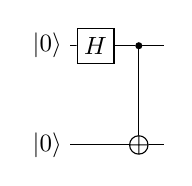
\begin{tikzpicture}[scale=0.9]
   \begin{yquant*}[register/minimum height=1.3cm]
   qubit {$\ket0$} x;
   qubit {$\ket0$} y;
   box {$H$} x;
   cnot y | x;
  \end{yquant*}
\end{tikzpicture}
\qquad\qquad
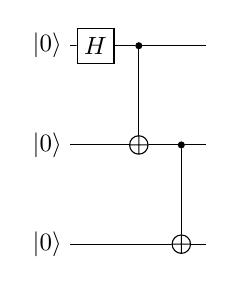
\begin{tikzpicture}[scale=0.9]
 \begin{yquant*}[register/minimum height=1.3cm]
   qubit {$\ket0$} x;
   qubit {$\ket0$} y;
   qubit {$\ket0$} z;
   box {$H$} x;
   cnot y | x;
   cnot z | y;
  \end{yquant*}
\end{tikzpicture}
\end{center}
\caption{\label{fig:bell2}Bell and GHZ States}
\end{figure}

Our observation is that a qubit in the special superposition
$1/\sqrt{2} ~(\ket{0} + \ket{1} )$ is, computationally speaking,
indistinguishable from a symbolic boolean variable with an unknown
value in the same sense used in symbolic evaluation of classical
programs. First, the superposition is not observable. The only way to
observe the qubit is via a measurement which collapses the state to be
either false or true with equal probability. Second, and more
significantly, this remarkably simple observation is quite robust even
in the presence of multiple, possibly entangled, qubits.

To see this, consider the conventional quantum circuits for creating
the maximally entangled Bell and GHZ states in
Fig.~\ref{fig:bell2}. On the left, the circuit generates the Bell
state $(1/\sqrt{2})~ (\ket{00} + \ket{11})$ as follows. First the state
evolves from $\ket{00}$ to $(1/\sqrt{2})~ (\ket{00} + \ket{10})$. Then
we apply the \cx-gate whose action is to negate the second qubit when
the first one is true. By using the symbol $x$ for $H\ket{0}$, the
input to the \cx-gate is $\ket{x0}$. A simple case analysis shows that
the action of \cx-gate on inputs $\ket{xy}$ is $\ket{x(x \oplus y)}$
where $\oplus$ is the exclusive-or boolean operation. In other words,
the \cx-gate transforms $\ket{x0}$ to $\ket{xx}$. Since any
measurement of the Bell state must produce either 00 or 11, 
a symbolic state that shares the same name in two positions
accurately represents the entangled Bell state. Similarly,
for the GHZ circuit on the right of Fig.~\ref{fig:bell2}, the state
after the Hadamard gate is $\ket{x00}$ which evolves to $\ket{xx0}$
and then to $\ket{xxx}$ again accurately capturing the entanglement
correlations.

\begin{figure*}[t]
  \centering
\begin{subfigure}[b]{.25\textwidth}
    \centering
    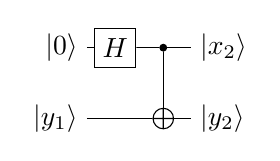
\begin{tikzpicture}[scale=1.0]
   \begin{yquant*}[register/minimum height=0.8cm]
   qubit {$\ket{0}$} x;
   qubit {$\ket{y_1}$} y;
   box {$H$} x;
   cnot y | x;
   output {$\ket{x_2}$} x;
   output {$\ket{y_2}$} y;
  \end{yquant*}
\end{tikzpicture}
\caption{\label{fig:bellqcore}Bell circuit}
\end{subfigure}
\qquad\qquad
\begin{subfigure}[b]{.25\textwidth}
    \centering
    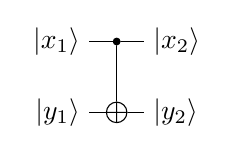
\begin{tikzpicture}[scale=1.0]
   \begin{yquant*}[register/minimum height=0.8cm]
   qubit {$\ket{x_1}$} x;
   qubit {$\ket{y_1}$} y;
   cnot y | x;
   output {$\ket{x_2}$} x;
   output {$\ket{y_2}$} y;
  \end{yquant*}
\end{tikzpicture}
\caption{\label{fig:bellccore}Symbolic variant}
\end{subfigure}
\caption{\label{fig:bellall}A conventional quantum circuit for
  generating a Bell state (a); its classical symbolic variant.}
\end{figure*}

Because quantum circuits are reversible, i.e., executable forwards
and backwards, the introduction of symbolic variables opens a host of
new exciting possibilities beyond conventional (classical) symbolic
evaluation: \emph{any mixture of inputs and outputs can be made
  symbolic}. For example, consider again the Bell circuit in
Fig.~\ref{fig:bellall} with an arbitrary initial value for the second
qubit. The right subfigure Fig.~\ref{fig:bellccore} removes the
explicit use of $H\ket{0}$ and replaces the top qubit with another
symbolic variable. Because quantum circuits are reversible, we can, at
this point, ``partially evaluate'' the circuit under various
regimes. For example, we can set $y_1=0$ and $y_2=1$ and ask about
values of $x_1$ and $x_2$ that would be consistent with this
setting. We can calculate backwards from $\ket{x_21}$ as follows. The
state evolves to $\ket{x_2(1 \oplus x_2)}$ which can be reconciled
with the initial conditions yielding the constraints $x_1=x_2$ and
$1 \oplus x_2 = 0$ whose solutions are $x_1 = x_2 = 1$.

\subsection*{Outline.}
We begin in Sec.~\ref{sec2} with background information covering the
special quantum circuits of interest and a review of boolean functions
and their algebraic normal form (ANF). Sec.~\ref{sec3} discusses the
main ideas of symbolic execution of these circuits in detail. Our main
contribution, the design and implementation, of a symbolic evaluator
for Hadamard-Toffoli quantum circuits, is explained in
Sec.~\ref{sec4}. The next section (Sec.~\ref{sec5}) includes a
complexity analysis and a performance evaluation of our symbolic
evaluator on major textbook algorithms. Sec.~\ref{sec6} concludes with
a summary and a discussion of the broader implications of our approach
to the understanding of the classical / quantum performance
characteristics. 


\begin{comment}

  eliminate superpositions
  use symbols to represent correlations in the quantum superposition
  H |0> replaced by x
  preserve the correlations in the quantum superposition but they are
    encoded in the correlations between symbols

  



There are three common ways to compute with \emph{unknown} values:
\begin{enumerate}
  \item by treating as symbolic variables,
  \item by using distributions,
  \item by using unitary operators (i.e. qubits).
\end{enumerate}
As a zeroth-order approximation, one can think of the ``unitary operators'' of quantum
computing as \Cplx-valued distributions. The extra ``phase'' involved allows tracking of
simple relations between inputs (i.e. \emph{entanglement}).

What we will do is to look at the classical reversible circuits at the heart
of quantum computation, replacing the qubits by symbolic quantities. We look at a particular
class of circuits with some \emph{inputs} and some \emph{ancillae} on one side, along
with some \emph{outputs} and the same ancillae restored to their initial values.

Furthermore, all the circuits look like ???

What a quantum circuit does with H on the ancilla is to transform a known input to
(the equivalent of) the uniform distribution on all possible values. The result is
basically \emph{maximally unknown}.

What we do instead is to remove the H, and treat the ancillae as dynamic inputs, i.e.
fully unknown. However, these circuits are all \emph{reversible}, so we can also 
start from a partial measurement (static), treating the rest of the state as dynamic.
We then execute the circuit backwards ``symbolically''.

While this sounds like the perfect setup for partial evaluation (PE) or slicing\footnote{
These are basically the same idea, but PE propagates known information forwards
through the program, and slicing propagates it backwards from the exit points}.
Since our circuits are reversible, for simplicity we're going to look at retrodictive
execution as forward execution of the reverse program, which puts us in the setup of PE.

Except that in PE, the result is a \emph{residual program} that obeys the Futumura equations.
In our case, we have ``both sides'', i.e. input, output and ancillae, in our hands. So the
result is going to be a set of equations constraining the ``possible pasts'' of the output
to be equal to the actual inputs. So rather than obtaining a residual program as output,
we obtain a \emph{system of equations}.

It all works because of two key things: we're only dealing with boolean values and with
circuits with operations (not, CX, CCX, and CCCX) that have simple symbolic forms.
Furthermore, boolean expressions (over AND and XOR) themselves have a normal form. So
we can propagate that through.

And now we give actual details.

Questions:
\begin{itemize}
  \item Where do we introduce the language over which we work (circuits)
\end{itemize}

Another try at 'the story'. (Parts done already deleted)
\begin{enumerate}
  \item measurements give us some knowledge of the output,
  \item this places us in a setting combining having forward static and
    dynamic knowledge of the input, in the context of a particular circuit,
    which is the domain of Partial Evalution (PE),
  \item this also places us in a setting combining having backward static and
    dynamic knowledge of the output, in the context of a particular circuit,
    which is the domain of Slicing,
  \item as the values we're dealing with (booleans) are simple, and the
    circuits only do simple, reversible operations, we can keep track of
    symbolic expressions for all values over the whole circuit. In other
    words, we never need to residualize a program, we get ``closed forms''
    representations (as boolean expressions),
  \item as we have knowledge forwards and backwards, the result of
    evaluation will be \emph{systems of constraints}.
  \item our test cases consist of circuits that form the heart \emph{classical},
    \emph{well-known} quantum circuits (Simon, \ldots, Shor)
  \item some of these circuits are extremely large, yet we process them quite
    quickly.
  \item The exact circuits we use are \emph{generalized Toffoli} gates (which
    are universal for reversible computation, and also ???)
  \item There exists a normal form for boolean functions ideally suited to our problem:
    ANF (\url{https://en.wikipedia.org/wiki/Algebraic_normal_form})
  \item evaluation on
    \begin{itemize}
      \item present test cases in more detail
      \item show results of running
        \begin{itemize}
          \item semantically
          \item timings
        \end{itemize}
    \end{itemize}
\end{enumerate}
\end{comment}

% So, all in all, I see the outline (and who seems in good position to write)
% \begin{enumerate}
%   \item Introduction [Amr]
%     \begin{itemize}
%       \item items 1-11 above, but 10-11 will be done in more depth later
%     \end{itemize}
% D \item Circuits and Boolean Functions [Jacques will try]
% D   \begin{itemize}
% D     \item redo 10 and 11 in more detail. Other background here
% D   \end{itemize}
%   \item Symbolic Evaluation of Circuits [Jacques]
%     \begin{itemize}
%       \item Define the problem we're tackling
%     \end{itemize}
% D \item Design and Implementation [Jacques]
% D   \begin{itemize}
% D     \item Give the design (lots of polymorphism, tagless, etc)
% D     \item Design of better data-structures for ANF
% D   \end{itemize}
%   \item Evaluation [Amr and Jacques]
%     \begin{itemize}
% D     \item Explain each of the circuits we're using [Jacques]
%       \item Explain how to 'read off' the answer from the constraints [Amr and Jacques]
%       \item Show some timings [Jacques]
%     \end{itemize}
%   \item Conclusion [?]
% \end{enumerate}

%%%%%%%%%%%%%%%%%%%%%%%%%%%%%%%%%%%%%%%%%%%%%%%%%%%%%%%%%%%%%%%%%%%%%%%%%
\section{Circuits and Boolean Functions}
\label{sec2}
 
\paragraph*{Special Circuits}
\begin{figure}[t]
  \begin{subfigure}{0.5\textwidth}
  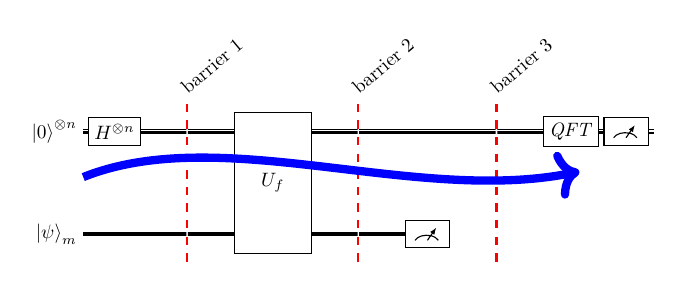
\begin{tikzpicture}[scale=0.7,every label/.style={rotate=40, anchor=south west}]
    \begin{yquant*}[operators/every barrier/.append style={red, thick},
        operator/minimum width=7mm,
        operator/separation=1mm,
        register/separation=10mm]
    qubits {$\ket0^{\otimes n}$} a;
    qubits {$\ket{\psi}_m$} b;
    box {$H^{\otimes n}$} a;
    ["barrier 1"]
    barrier (-);
    [x radius=7mm, y radius=7mm]
    box {$U_f$} (a,b);
    ["barrier 2"]
    barrier (-);
    measure b;
    discard b;
    ["barrier 3"]
    barrier (-);
    box {$\mathit{QFT}$} a;
    measure a;
    \end{yquant*}
    \draw[line width=3pt, ->, blue] (0,-1.1) .. controls (2.5,-0.1) and (6,-1.6) .. (9,-1);
  \end{tikzpicture}
  \caption{Conventional Flow}
  \end{subfigure}
  \begin{subfigure}{0.5\textwidth}
  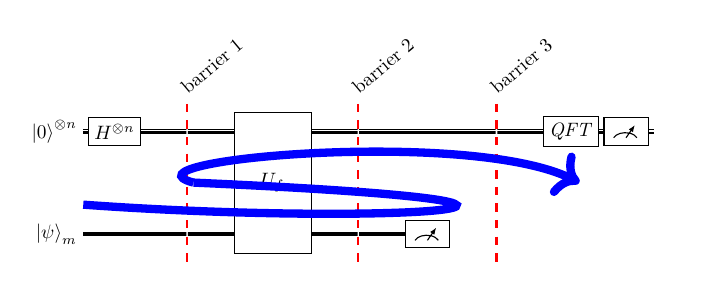
\begin{tikzpicture}[scale=0.7,every label/.style={rotate=40, anchor=south west}]
    \begin{yquant*}[operators/every barrier/.append style={red, thick},
        operator/minimum width=7mm,
        operator/separation=1mm,
        register/separation=10mm]
    qubits {$\ket0^{\otimes n}$} a;
    qubits {$\ket{\psi}_m$} b;
    box {$H^{\otimes n}$} a;
    ["barrier 1"]
    barrier (-);
    [x radius=7mm, y radius=7mm]
    box {$U_f$} (a,b);
    ["barrier 2"]
    barrier (-);
    measure b;
    discard b;
    ["barrier 3"]
    barrier (-);
    box {$\mathit{QFT}$} a;
    measure a;
  \end{yquant*}
  \draw[line width=3pt, blue] (0,-1.6) .. controls (5.5,-2) and (11,-1.6) .. (2,-1.2);
  \draw[line width=3pt, ->, blue] (2,-1.2) .. controls (0.5,-0.8) and (7,-0.2) .. (9,-1.2);
  \end{tikzpicture}
  \caption{Retrodictive Flow}
  \end{subfigure}
\caption{\label{fig:templateQC}Template quantum circuit}
\end{figure}

We analyze a particular class of circuits, namely those
that match the template in Fig.~\ref{fig:templateQC} (including
Deutsch, Deutsch-Jozsa, Bernstein-Vazirani, Simon, Grover, and Shor's
algorithms~\cite{doi:10.1137/S0097539796300921,deutsch,deutschJozsa,365701,doi:10.1137/S0097539795293172,nielsen_chuang_2010,10.1145/237814.237866}). 
The $U_f$ block, defined as 
\begin{equation}
  U_f(\ket{x}\ket{y}) = \ket{x}\ket{f(x) \oplus y},
\end{equation}
ends up being completely classical, albeit performing mixed mode
execution of the circuit. More precisely, here it means that in
all these algorithms, the top collection of wires (which we will call
the computational register) is prepared in a uniform superposition
which can be represented using symbolic variables. The measurement of
the bottom collection of wires (which we call the ancilla register)
after barrier 2 provides partial information about the future which
is, together with the initial conditions of the ancilla register,
sufficient to symbolically execute the circuit. In each case, instead
of the conventional execution flow depicted in
Fig.~\ref{fig:templateQC}(a), we find a possible measurement outcome
$w$ at barrier (2) and perform a symbolic retrodictive execution with
a state $\ket{xw}$ going backwards to collect the constraints on $x$
that enable us to solve the problem in question.

\begin{figure}[t]
  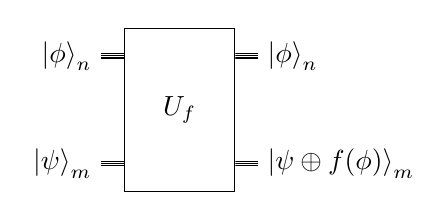
\begin{tikzpicture}[every label/.style={rotate=40, anchor=south west}]
    \begin{yquant*}[
        operator/minimum width=7mm,
        operator/separation=3mm,
        register/separation=10mm]
    qubits {$\ket{\phi}_n$} a;
    qubits {$\ket{\psi}_m$} b;
    [x radius=7mm, y radius=7mm]
    box {$U_f$} (a,b);
    output {$\ket{\phi}_n$} a;
    output {$\ket{\psi \oplus f(\phi)}_m$} b;
    \end{yquant*}
  \end{tikzpicture}
\caption{\label{fig:CircuitAbstraction}Circuit Abstraction}
\end{figure}

In other words, it suffices to look at circuits that match the
template in Fig.~\ref{fig:CircuitAbstraction}.

\paragraph*{Algebraic Normal Form (ANF).}

Furthermore, the circuits we are interested in can all be expressed
in terms of \emph{generalized Toffoli gates} with $n$ control qubits:
$a_{n},\cdots,a_0$ and one target qubit $c$ is $c \oplus \bigwedge_i
a_i$, the exclusive-or of the target $c$ with the conjunction of all
the control qubits. In fact, we generalize this further, so that we
can control either on a qubit or its negation, by using pairs of
control qubit and a boolean. In other words, our gates are
$(a_{n}, b_{n}),\cdots,(a_0,b_0)$ and one target qubit $c$ is 
$c \oplus \bigwedge_i \left(a_i == b_i\right)$, the exclusive-or of the 
target $c$ with the conjunction of the result of testing each qubit
against its corresponding target boolean. Note that
$\left(a_i == 1\right)$ can be expressed as just $a_i$, and
$\left(a_i == 0\right)$ can be expressed as $1 \oplus a_i$.
Such generalized Toffoli gates with $n$ control qubits are called
$c^nx$ gates. The special cases
for $n=0$ is the \emph{not} gate 'x', 
for $n=1$ is the \emph{controlled not} gate 'cx', and
for $n=2$ is the classical \emph{Toffoli} gate 'ccx'.

The \emph{algebraic normal form} 
(also called ring sum normal form, Zhegalkin normal form or
Reed-Muller expansion)
of boolean functions $\Bool^n\rightarrow\Bool$
is as the exclusive-or ($\oplus$) of ands ($\wedge$) of $0$ or more
of the inputs $x_i$. Note that the and of $0$ inputs is $1$. It is then
easy to see that generalized Toffoli gates (without the extra boolean) are
already in algebraic normal form.
Furthermore, circuits that only
use \x\ and \cx-gates never generate any conjunctions and hence lead
to formulae that are efficiently solvable
classically~\cite{10.5555/35517,TOKAREVA20151}.

%%%%%%%%%%%%%%%%%%%%%%%%%%%%%%%%%%%%%%%%%%%%%%%%%%%%%%%%%%%%%%%%%%%%%%%%% 

\section{Symbolic Evaluation of Circuits}
\label{sec3}

Our problem then reduces to a mixture of partial evaluation, slicing
and symbolic evaluation. Like with partial evaluation, we have some
inputs dynamic, some static, and a static program. Similarly for slicing,
but with outputs. Our situation is significantly simpler than in both
cases. First, our language is reversible, which makes backwards evaluation
deterministic, unlike for most languages. Second, the values at each step
of circuit execution are boolean functions, and thus expressible in ANF.

Thus we never need to residualize a circuit, we can always get a ``closed
form'', in ANF, for evaluation, whether forward or backward. In the
\emph{retrodictive} mode of running our circuits, we take a combination
of static and dynamic knowledge of the output, run the circuit backwards,
and produce as output a \emph{system of constraints} equating the resulting
logical polynomials to the circuit's inputs. If the system of constraints
has a solution, then that output was feasible. 

It's important to note that our circuits are given as white boxes. In 
particular, the $b_i$ are circuit constants, so we can always express
everything in algebrais normal form.

What we will then see is that for many classical circuits, we can
``read off'' the information we need from the system of constraint themselves,
\emph{without needing to actually solve them}.

%%%%%%%%%%%%%%%%%%%%%%%%%%%%%%%%%%%%%%%%%%%%%%%%%%%%%%%%%%%%%%%%%%%%%%%%% 
\section{Design and Implementation}
\label{sec4}

Our exposition of the design and implementation of our system will
follow Parnas' advice on \emph{faking it}~\cite{ParnasFake}: a reconstruction
of the requirements as we should have had them if we'd been all-knowing,
and a design that fits those requirements. The version history in our github
repository can be inspected for anyone who wants to see our actual path.

As we experimented with the idea of partial evaluation and symbolic
execution of circuits, we ended up writing a lot of variants of
essentially the same code, but with minor differences in representation.
From these early experiments, we could see the major variation points:
\begin{itemize}
  \item representation of \emph{boolean values} and \emph{boolean functions},
  \item representation of ANF,
  \item representation of circuits.
\end{itemize}
We also wanted to write out circuits only once, and have them be valid
across these representation changes.

A number of our examples involve arbitrary boolean functions (given as black
boxes at ``compile time'') for which we want to, offline, generate an
equivalent reversible circuit. In other words for $f : \Bool^n \rightarrow\Bool$,
we wish to generate the circuit for $g : \Bool^{n+1} \rightarrow \Bool^{n+1}$ such
that for $\overline{x} : \Bool^n$, then 
$g(\overline{x},y) = (\overline{x}, y \oplus f(\overline{x}))$.

This leads us to the requirements our code must fulfill.

\begin{figure*}[t]
\begin{tabular}{l | p{13cm}}
  \textbf{Module} & \textbf{Service} \\ \hline
  \texttt{Value} & representation of a \emph{language of values}
    (as a typeclass) and some constructors\\
  \texttt{FormulaRepr} & abstract representation of formulas, as
    a mapping from abstract variables to abstract formulas\\
  \texttt{Variable} & variables as locations holding values and
    their constructors\\
  \texttt{ModularArith} & modular arithmetic utilities useful in
    implementing certain algorithms, like Shor's\\
  \texttt{BoolUtils} & function to interpret a list of booleans as
    an Integer\\
  \texttt{GToffoli} & representation of generalized Toffoli gates
    and some constructors\\
  \texttt{Circuits} & representation of circuits (sequences of gates)
    and of the special ``wires'' of our circuits\\
  \texttt{Synthesis} & synthesis algorithm for circuits with particular
    properties\\
  \texttt{ArithCirc} & creation of arithmetic circuits\\
  \texttt{EvalZ} & evaluation of circuits on concrete values\\
  \texttt{FormAsList} & representation of formulas as xor-lists 
    of and-lists of literals-as-strings\\
  \texttt{FormAsMaps} & representation of formulas as xor-maps
    of and-maps of literals-as-Int\\
  \texttt{FormAsBitmaps} & representation of formulas as xor-maps
    of bitmaps\\
  \texttt{SymbEval} & Symbolic evaluation of circuits\\
  \texttt{SymbEvalSpecialized} & Symbolic evaluation of circuits
    specialized to the representation from \texttt{FormAsBitmaps}\\
  \texttt{QAlgos} & generating the circuits themselves\\
  \texttt{RunQAlgos} & running the actual circuits \\
  \texttt{Trace} & utilities for tracing and debugging 
\end{tabular}
  \caption{Modules and their services}
  \label{fig:modules}
\end{figure*}

\subsection{Requirements}

We need to be able to deal with the following variabilities:
\begin{enumerate}
  \item multiple representations of \emph{boolean values},
  \item multiple representations of \emph{boolean formulas},
  \item different evaluation means (directly and symbolically),
\end{enumerate}

\noindent It must also be possible to implement the following:
\begin{enumerate}[resume]
  \item a reusable representation of circuits composed of generalized Toffoli gates,
  \item a reusable representation of the inputs, outputs and ancillae associated to
    a circuit,
  \item a \emph{synthesis} algorithm for circuits implementing a certain boolean
    function,
  \item a reusable library of circuits (such as
    Deutsch, Deutsch-Jozsa, Bernstein-Vazirani, Simon, Grover, and Shor). 
\end{enumerate}
\noindent From those, we can make a
set of design choices that drive the eventual solution.

We eventually want some non-functional characteristics to hold:
\begin{enumerate}[resume]
  \item evaluation of reasonably-sized circuits should be relatively efficient.
\end{enumerate}

\subsection{Design}

To meet the first requirement, we use \emph{finally tagless}~\cite{tagless}
to encode a \emph{language of values}:
\begin{minted}{haskell}
  class (Show v, Enum v) => Value v where
  zero :: v
  one  :: v
  snot :: v -> v
  sand :: v -> v -> v
  sxor :: v -> v -> v

  -- has a default implementation
  snand :: [v] -> v -- n-ary and
  snand = foldr sand one
\end{minted}
\noindent which is then implemented $4$ times, once for $\texttt{Bool}$
and then multiple times for different symbolic variations. As a side-effect,
this gives us requirement $3$ ``for free'' if we can write a sufficiently
polymorphic evaluator (which we will present below).

Unlike for value representation which can be computed from context, we want
to explicitly choose formula representation (requirement 2) ourselves. Thus we
use an explicit record instead of an implicit dictionary:
\begin{minted}{haskell}
data FormulaRepr f r = FR 
  { fromVar  :: r -> f
  , fromVars :: Int -> r -> [ f ]
  }
\end{minted}
\noindent The main methods are about \emph{variable representation} \texttt{r}
and how to insert them into the current \emph{formula representation} \texttt{f},
singly or $n$ at once.

A Generalized Toffoli gates can be represented by a list of representation of
value accessors \texttt{br} (short for boolean representation) along with a list
of \emph{controls} that tell us whether to use the bit directly or negated,
along with which value will potentially be flipped. The implementation of very 
common gates (negation and controlled not) are also shown.
\begin{minted}{haskell}
data GToffoli br = GToffoli [Bool] [br] br

xop :: br -> GToffoli br
xop = GToffoli [] []

cx :: br -> br -> GToffoli br
cx a = GToffoli [True] [a]
\end{minted}
\noindent The core of a circuit (requirement $4$) is then implemented as a 
sequence of these (where \texttt{Seq} is from {Data.Sequence}).
\begin{minted}{haskell}
type OP br = Seq (GToffoli br)
\end{minted}

\noindent Mainly for efficiency reasons, we model circuits as manipulating
\emph{locations holding values} rather than directly acting on values. We
use \texttt{STRef}s (aliased to \texttt{Var}) for that purpose. Putting this
together with the model of circuits of \ref{sec:circuitmodel}, we get
\begin{minted}{haskell}
data Circuit s v = Circuit
  { op          :: OP (Var s v)
  , xs          :: [Var s v]
  , ancillaIns  :: [Var s v]
  , ancillaOuts :: [Var s v]  
  , ancillaVals :: [v]
  }
\end{minted}
\noindent which lets us achieve requirement $5$.

For requirement $6$, we implement a straightforward version of 
the algorithm of~\cite{SoekenEtAl2016}. Our implementation is
\emph{language agnostic}, in other words it works via the \texttt{Value}
interface, so that the resulting circuits are all of type \texttt{OP br}
for a free representation \texttt{br}. As circuit synthesis is only
done for generating examples, we are not worried about its efficiency.

The arithmetic circuit generators are also based on classical algorithms, and are
not optimized in any way, neither for running time nor for gate count. Neither are
the code for the classical quantum algorithms. They are, however, representation
polymorphic.

Above, we said we had $3$ different symbolic evaluators. These were not driven
by having different levels of \emph{precision} but rather by requirement $8$,
efficiency. Our first evaluator (\texttt{FormAsList}) uses xor-lists of
and-lists of literals (as strings, i.e.
\texttt{"x0"}, \texttt{"x1"}, \ldots in lexicographical order of the wires). ANF 
is then easy: and-lists are sorted, and duplicates removed. Xor-lists are sorted,
grouped, even length lists are removed, and then made unique. This is woefully
inefficient, and was the clear bottleneck in our profiles.

A less na\"{\i}ve approach uses a set of bits for representing literals, an
\texttt{IntSet} for and-lists, and a normalized multiset for xor maps. We found
more efficient to use a multiset for intermediate computations with xor maps
which is normalized at the end instead of trying to track even/odd number of
occurrences. Only computing Cartesian products in this representation requires
some thought for finding a reasonably efficient algorithm.

While significantly faster, this was still not sufficiently efficient. Our final
representation uses Natural numbers as and-maps where the encoding of literals is
now positional, and xor maps are again multisets of these ``bitmaps''.

As a last optimization, our circuits have a very particular property: the control
wires are not written to, so that they are all literals. This can be used to
further optimize the evaluation of single gates.

\subsection{Implementation}

The final code consists of $18$ modules that implement various
services, see Fig.~\ref{fig:modules} for a full listing. It consists of
only $1449$ lines of Haskell code, of which $646$ lines are blank, import or
comments, module declaration, so that $809$ are ``code''. Testing and printing
utilities are not counted in the above.

The code that occupies the most volume is that for running the examples, as each
circuit needs its own setup for the input and ancilla wires. Next is the implementation
of symbolic representations of formulas in ANF. This is largely because there are a
lot of pieces that need to be defined, including many instances; the algorithmic aspect
rarely span more than $15$ lines in total. The code for generating arithmetic circuits
is voluminous as well as largely computational, but is a re-implementation of known
material, as is the synthesis code.

A few comments on further implementation details. Sharp readers might have noticed
\texttt{snand} as defined in class \texttt{Value} instead of as a polymorphic function
outside the class; we do this to enable its implementation to be overridden.
Lastly, \texttt{GToffoli}'s implementation relies on an unexpressed invariant: that its
two lists are of equal length. We really ought to refactor the code to use a single
list of tuples, but this is a pervasive change that would not bring much benefit as
we use combinators to build circuits, and these already maintain that invariant.
Similarly for \texttt{Circuit}: the lists \texttt{ancillaIns}, \texttt{ancillaOut}
and \texttt{ancillaVals} should all be of the same length. That invariant is not
checked in our code.

%%%%%%%%%%%%%%%%%%%%%%%%%%%%%%%%%%%%%%%%%%%%%%%%%%%%%%%%%%%%%%%%%%%%%%%%% 

\section{Evaluation}
\label{sec5}

We implement six well-known quantum algorithms: 
Deutsch, Deutsch-Jozsa, Bernstein-Vazirani, Simon, Grover, and Shor. 
We first define all six, then explain interesting aspects of running them.

\subsection{The Algorithms.} 

\begin{comment}
  % Jacques: I don't find this circuit brings much to the discussion.
\begin{figure}[ht]
  \centering
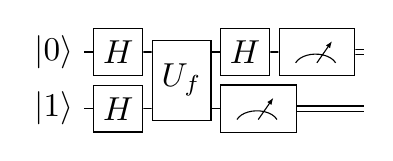
\begin{tikzpicture}[scale=1.2]
   \begin{yquant*}
   qubit {$\ket0$} x;
   qubit {$\ket1$} y;
   box {$H$} x;
   box {$H$} y;
   box {$U_f$} (x,y);
   measure y;
   box {$H$} x;
   measure x;
  \end{yquant*}
\end{tikzpicture}
\caption{\label{fig:deutsch}Quantum Circuit for the Deutsch-Jozsa
  Algorithm $(n=1)$}
\end{figure}
\end{comment}

Let $\finset{n}$ denote the finite set $\{ 0,1,\ldots,(n-1)\}$. The
parameter $n$ determines the problem size in all the problems below
(except Deutsch which is a fixed sized problem).

\paragraph*{Deutsch.}
The conventional statement of the problem is to determine if a
function $\finset{2} \rightarrow \finset{2}$ is constant or
balanced. An equivalent statement is to answer a query about the
cardinality of a pre-image. In this case, if the cardinality of the
pre-image of any value in the range is even i.e. 0 or 2, the function
must be constant and if it is odd, i.e., it contains just one element,
the function must be balanced.

\paragraph*{Deutsch-Jozsa.}
The problem is a generalization of the previous one: the question is
to determine if a function $\finset{2^n} \rightarrow \finset{2}$ for
some $n$ is constant or balanced. When expressed as a pre-image
computation, the problem reduces to a query distinguishing the
following three situations about the pre-image of a value in the range
of the function: is the cardinality of the pre-image equal to 0,
$2^n$, or $2^{n-1}$? In the first two cases, the function is constant
and in the last case, the pre-image contains half the values in the
domain indicating that the function is balanced.

\paragraph*{Bernstein-Vazirani.}
We are given a function $f : \finset{2^n} \rightarrow \finset{2}$
that hides a secret number $s \in \finset{2^n}$. We are promised the
function is defined using the binary representations $\sum_i^{n-1}
x_i$ and $\sum_i^{n-1} s_i$ of $x$ and $s$ respectively as follows:
\[
f(x) = \sum_{i=0}^{n-1} s_ix_i \mod{2}
\]
The goal is to determine the secret number $s$. 

Expressing the problem as a pre-image calculation is slightly more
involved than in the previous two cases. To determine $s$, we make $n$
queries to the pre-image of a value in the range of the
function. Query $i$ asks whether $2^i$ is a member of the pre-image
and the answer determines bit $i$ of the secret $s$. Indeed, by
definition, $f(2^i) = s_i$ and hence $s_i$ is 1 iff $2^i$ is a member
of the pre-image of 1.

\paragraph*{Bernstein-Vazirani.}
We are given a function $f : \finset{2^n} \rightarrow \finset{2}$
that hides a secret number $s \in \finset{2^n}$. We are promised the
function is defined using the binary representations $\sum_i^{n-1}
x_i$ and $\sum_i^{n-1} s_i$ of $x$ and $s$ respectively as follows:
\[
f(x) = \sum_{i=0}^{n-1} s_ix_i \mod{2}
\]
The goal is to determine the secret number $s$. 

Expressing the problem as a pre-image calculation is slightly more
involved than in the previous two cases. To determine $s$, we make $n$
queries to the pre-image of a value in the range of the
function. Query $i$ asks whether $2^i$ is a member of the pre-image
and the answer determines bit $i$ of the secret $s$. Indeed, by
definition, $f(2^i) = s_i$ and hence $s_i$ is 1 iff $2^i$ is a member
of the pre-image of 1.

\paragraph*{Simon.}
We are given a 2-1 function $f : \finset{2^n} \rightarrow
\finset{2^n}$ with the property that there exists an $a$ such $f(x) =
f(x \oplus a)$ for all~$x$; the goal is to determine $a$. When
expressed as a computation of pre-images, the problem statement
becomes the following. Pick an arbitrary $x$ and compute the pre-image
of $f(x)$. It must contain exactly two values one of which is $x$. The
problem then reduces to finding the other value in the pre-image.

\paragraph*{Grover}
We are given a function $f : \finset{2^n} \rightarrow \finset{2}$
such that there is a unique $u \in \finset{2^n}$ such that $f(u)=1$.
The problem is to find this $u$.

\paragraph*{Shor.}
The quantum core of the algorithm is the following. We are given a
periodic function $f(x) = a^x \mod{2^n}$ and the goal is to determine
the period. As a computation over pre-images, the problem can be
recast as follows. For an arbitrary $x$, compute the pre-image of
$f(x)$ and query it to determine the period.

\subsection{Running the Algorithms}

\paragraph*{Deutsch and Deutsch-Jozsa}
Instead
of the conventional execution, we perform a retrodictive execution of
the $U_f$ block with an ancilla measurement~$0$, i.e., with the state
$\ket{x_{n-1}\cdots x_1x_00}$.  The result of the execution is a
symbolic formula $r$ that determines the conditions under which
$f(x_{n-1},\cdots,x_0) = 0$. When the function is constant, the
results are $0=0$ (always) or $1=0$ (never). When the function is
balanced, we get a formula that mentions the relevant variables. For
example, here are the results of three executions for balanced
functions $\finset{2^6} \rightarrow \finset{2}$:
\begin{itemize}
\item $x_0 = 0$,
\item $x_0 \oplus x_1 \oplus x_2 \oplus x_3 \oplus
    x_4 \oplus x_5 = 0$, and
\item $1 \oplus x_3x_5 \oplus x_2x_4 \oplus x_1x_5
\oplus x_0x_3 \oplus x_0x_2 \oplus x_3x_4x_5 \oplus x_2x_3x_5 \oplus
x_1x_3x_5 \oplus x_0x_3x_5 \oplus x_0x_1x_4 \oplus x_0x_1x_2 \oplus
x_2x_3x_4x_5 \oplus x_1x_3x_4x_5 \oplus x_1x_2x_4x_5 \oplus
x_1x_2x_3x_5 \oplus x_0x_3x_4x_5 \oplus x_0x_2x_4x_5 \oplus
x_0x_2x_3x_5 \oplus x_0x_1x_4x_5 \oplus x_0x_1x_3x_5 \oplus
x_0x_1x_3x_4 \oplus x_0x_1x_2x_4 \oplus x_0x_1x_2x_4x_5 \oplus
x_0x_1x_2x_3x_5 \oplus x_0x_1x_2x_3x_4 = 0$.
\end{itemize}
In the first case, the function is balanced because it produces $0$
exactly when $x_0=0$ which happens half of the time in all possible
inputs; in the second case the output of the function is the
exclusive-or of all the input variables which is another easy instance
of a balanced function. The last case is a cryptographically strong
balanced function whose output pattern is balanced but, by design,
difficult to discern~\cite{quteprints21763}.

An important insight is that we actually do not care about the exact
formula. Indeed, since we are \emph{promised} that the function is either
constant or balanced, then any formula that refers to at least one
variable must indicate a balanced function. In other words, the
outcome of the algorithm can be immediately decided if the formula is
anything other than 0 or 1. Indeed, our implementation correctly
identifies all 12870 balanced functions $\finset{2^4} \rightarrow
\finset{2}$. This is significant as some of these functions produce
complicated entangled patterns during quantum evolution and could not
be de-quantized using previous approaches~\cite{djdeq}. 
However, it is important to remember that are circuits are ``white-box''
rather than ``black-box'', which yields a very different complexity
model~\cite{10.1145/3341106}.

\begin{figure*}
\begin{tabular}{ll}
$u=0$ & 
  $\red{1} \oplus x_3 \oplus x_2 \oplus x_1 \oplus x_0 \oplus x_2x_3 \oplus x_1x_3 \oplus x_1x_2 \oplus x_0x_3 \oplus x_0x_2 \oplus x_0x_1 \oplus x_1x_2x_3 \oplus x_0x_2x_3$ \\
   &\quad $\oplus ~x_0x_1x_3 \oplus x_0x_1x_2 \oplus x_0x_1x_2x_3$ \\
$u=1$ & 
  $\red{x_0} \oplus x_0x_3 \oplus x_0x_2 \oplus x_0x_1 \oplus x_0x_2x_3 \oplus x_0x_1x_3 \oplus x_0x_1x_2 \oplus x_0x_1x_2x_3$ \\
$u=2$ &
  $\red{x_1} \oplus x_1x_3 \oplus x_1x_2 \oplus x_0x_1 \oplus x_1x_2x_3 \oplus x_0x_1x_3 \oplus x_0x_1x_2 \oplus x_0x_1x_2x_3$ \\
$u=3$ &
  $\red{x_0x_1} \oplus x_0x_1x_3 \oplus x_0x_1x_2 \oplus x_0x_1x_2x_3$ \\
$u=4$ &
  $\red{x_2} \oplus x_2x_3 \oplus x_1x_2 \oplus x_0x_2 \oplus x_1x_2x_3 \oplus x_0x_2x_3 \oplus x_0x_1x_2 \oplus x_0x_1x_2x_3$ \\
$u=5$ &
  $\red{x_0x_2} \oplus x_0x_2x_3 \oplus x_0x_1x_2 \oplus x_0x_1x_2x_3$ \\
$u=6$ &
  $\red{x_1x_2} \oplus x_1x_2x_3 \oplus x_0x_1x_2 \oplus x_0x_1x_2x_3$ \\
$u=7$ &
  $\red{x_0x_1x_2} \oplus x_0x_1x_2x_3$ \\
$u=8$ &
  $\red{x_3} \oplus x_2x_3 \oplus x_1x_3 \oplus x_0x_3 \oplus x_1x_2x_3 \oplus x_0x_2x_3 \oplus x_0x_1x_3 \oplus x_0x_1x_2x_3$ \\
$u=9$ &
  $\red{x_0x_3} \oplus x_0x_2x_3 \oplus x_0x_1x_3 \oplus x_0x_1x_2x_3$ \\
$u=10$ &
  $\red{x_1x_3} \oplus x_1x_2x_3 \oplus x_0x_1x_3 \oplus x_0x_1x_2x_3$ \\
$u=11$ &
  $\red{x_0x_1x_3} \oplus x_0x_1x_2x_3$ \\
$u=12$ &
  $\red{x_2x_3} \oplus x_1x_2x_3 \oplus x_0x_2x_3 \oplus x_0x_1x_2x_3$ \\
$u=13$ &
  $\red{x_0x_2x_3} \oplus x_0x_1x_2x_3$ \\
$u=14$ &
  $\red{x_1x_2x_3} \oplus x_0x_1x_2x_3$ \\
$u=15$ &
  $\red{x_0x_1x_2x_3}$
\end{tabular}
\caption{\label{fig:Grover}Result of retrodictive execution for the Grover oracle ($n=4$, $w$ in the range $\{0..15\}$). The highlighted red subformula is the binary representation of the hidden input $u$.}
\end{figure*}

\paragraph*{Bernstein-Vazirani}

\paragraph*{Grover}

\paragraph*{Simon}

The discussion above suggests that the details of the equations may
not be particularly relevant for some algorithms. This would be
crucial as the satisfiability of general boolean equations is, in
general, an $\mathit{NP}$-complete
problem~\cite{4640789,Karp1972,10.1145/800157.805047}. Fortunately,
this observation does hold for other algorithms as well including the
Bernstein-Vazirani algorithm and Grover's algorithm. In both cases,
the result can be immediately read from the formula. In the
Bernstein-Vazirani case, formulae are guaranteed to be of the form
$x_1 \oplus x_3 \oplus x_4 \oplus x_5$; the secret string is then the
binary number that has a 1 at the indices of the relevant variables
$\{ 1,3,4,5 \}$. In the case for Grover, because there is a unique
input $u$ for which $f(u) = 1$, the ANF formula must include a
subformula matching the binary representation of $u$, and in fact that
subformula is guaranteed to be the shortest one as shown in
Fig.~\ref{fig:Grover}.

\begin{figure*}
\[\begin{array}{l@{\quad}lllll}
\textrm{Base} & \multicolumn{4}{c}{\textrm{Equations}} & \textrm{Solution} \\[2ex]
a=11 & x_0 = 0 &&&& \red{x_0 = 0} \\
a=4,14 & 1 \oplus x_0 = 1 & x_0 = 0 &&
  & \red{x_0 = 0} \\
a=7,13 & 1 \oplus x_1 \oplus x_0x_1 = 1 & x_0x_1 = 0 & x_0 \oplus x_1 \oplus x_0x_1 = 0 &  x_0 \oplus x_0x_1 = 0 & \red{x_0=x_1=0} \\
a=2,8 & 1 \oplus x_0 \oplus x_1 \oplus x_0x_1 = 1 & x_0x_1 = 0 & x_1 \oplus x_0x_1 = 0 & x_0 \oplus x_0x_1 = 0  & \red{x_0=x_1=0}
\end{array}\]
\caption{\label{fig:shor-eqs}Equations generated by retrodictive
  execution of $a^x \mod{15}$ for different values of $a$, starting
  from observed result 1 and unknown
  $x_8x_7x_6x_5x_4x_3x_2x_1x_0$. The solution for the unknown
  variables is given in the last column.}
\end{figure*}

\begin{figure}{r}
\begin{center}
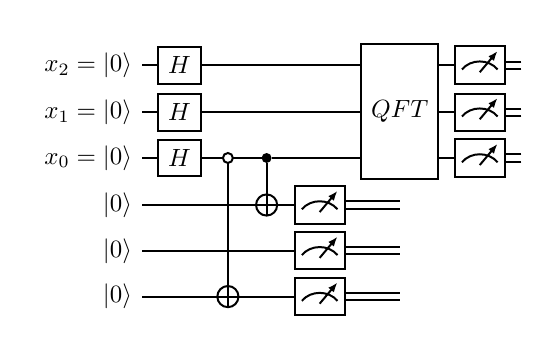
\begin{tikzpicture}
\node[scale=0.9]{    
\begin{quantikz}[row sep=0.005cm,column sep=0.22cm]
\lstick{$x_2 = \ket{0}$} & \gate{H}& \qw & \qw 
      & \qw & \gate[wires=3][0.5cm]{QFT} & \meter{} & \cw \\
\lstick{$x_1 = \ket{0}$} & \gate{H} & \qw & \qw       
      & \qw & & \meter{} & \cw \\
\lstick{$x_0 = \ket{0}$} & \gate{H} & \octrl{3} & \ctrl{1}
      & \qw & & \meter{} & \cw \\
\lstick{$\ket{0}$} & \qw & \qw & \targ{}
      & \meter{} & \cw \\
\lstick{$\ket{0}$} & \qw & \qw  & \qw
      & \meter{} & \cw \\
\lstick{$\ket{0}$} & \qw & \targ{} & \qw 
      & \meter{} & \cw
\end{quantikz}
};\end{tikzpicture}
\end{center}
\caption{\label{fig:shor15}Finding the period of $4^x \mod{15}$}
\end{figure}
\paragraph*{Shor}
The circuit in Fig.~\ref{fig:shor15} uses a hand-optimized
implementation of quantum oracle $U_f$ for the modular exponentiation
function $f(x) = 4^x \mod{15}$ to factor 15 using Shor's
algorithm. The white dot in the graphical representation of the first
indicates that the control is active when it is 0. In a conventional
forward execution, the state before the QFT block is:
\[
\frac{1}{2\sqrt{2}} (
  (\ket{0} + \ket{2} + \ket{4} + \ket{6}) \ket{1} + 
  (\ket{1} + \ket{3} + \ket{5} + \ket{7}) \ket{4}
  )
\]
At this point, the ancilla register is measured to either $\ket{1}$ or
$\ket{4}$. In either case, the computational register snaps to a state
of the form $\sum_{r=0}^3 \ket{a+2r}$ whose QFT has peaks at $\ket{0}$
or $\ket{4}$ making them the most likely outcomes of measurements of
the computational register. If we measure $\ket{0}$, we repeat the
experiment; otherwise we infer that the period is~2.

In the retrodictive execution, we can start with the state
$\ket{x_2x_1x_0001}$ since 1 is guaranteed to be a possible ancilla
measurement (corresponding to $f(0)$). The first \cx-gate changes the
state to $\ket{x_2x_1x_0x_001}$ and the second \cx-gate produces
$\ket{x_2x_1x_0x_00x_0}$. At that point, we reconcile the retrodictive
result of the ancilla register $\ket{x_00x_0}$ with the initial
condition $\ket{000}$ to conclude that $x_0=0$. In other words, in
order to observe the ancilla at $001$, the computational register must
be initialized to a superposition of the form $\ket{??0}$ where the
least significant bit must be 0 and the other two bits are
unconstrained. Expanding the possibilities, the first register needs
to be in a superposition of the states $\ket{000}, \ket{010},
\ket{100}$ or $\ket{110}$ and we have just inferred using purely
classical but retrodictive reasoning that the period is
2.

This result does not, in fact, require the small optimized circuit of
Fig.~\ref{fig:shor15}. In our implementation, modular exponentiation
circuits are constructed from first principles using adders and
multipliers~\cite{PhysRevA.54.147}. In the case of $f(x) = 4^x
\mod{15}$, although the unoptimized constructed circuit has 56,538
generalized Toffoli gates (controlled$^{n}$-not gates for all $n$),
the execution results in just two simple equations: $x_0 = 0$ and $1
\oplus x_0 = 1$. Furthermore, as shown in Fig.~\ref{fig:shor-eqs}, the
shape and size of the equations is largely insensitive to the choice
of 4 as the base of the exponent, leading in all cases to the
immediate conclusion that the period is either 2 or 4. When the
solution is $x_0=0$, the period is 2, and when it is $x_0=x_1=0$, the
period is~4.

The remarkable effectiveness of retrodictive computation of the Shor
instance for factoring 15 is due to a coincidence: a period that is a
power of 2 is clearly trivial to represent in the binary number system
which, after all is expressly designed for that purpose. That
coincidence repeats itself when factoring products of the (known)
Fermat primes: 3, 5, 17, 257, and 65537, and leads to small
circuits~\cite{shorFermat}. This is confirmed with our implementation
which smoothly deals with unoptimized circuits for factoring such
products. Factoring 3*17=51 using the unoptimized circuit of 177,450
generalized Toffoli gates produces just the 4 equations: $1 \oplus x_1
= 1$, $x_0 = 0$, $x_0 \oplus x_0x_1 = 0$, and $x_1 \oplus x0x1 =
0$. Even for 3*65537=196611 whose circuit has 4,328,778 generalized
Toffoli gates, the execution produces 16 small equations that refer to
just the four variables $x_0$, $x_1$, $x_2$, and $x_3$ constraining
them to be all 0, i.e., asserting that the period is 16.

\begin{figure}
  \centering
    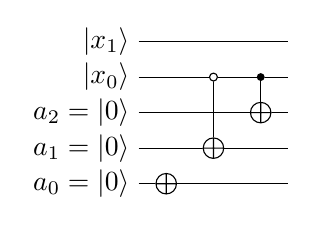
\begin{tikzpicture}[scale=1.0]
   \begin{yquant*}
   qubit {$\ket{x_1}$} x1;
   qubit {$\ket{x_0}$} x0;
   qubit {$a_2 = \ket0$} a2;
   qubit {$a_1 = \ket0$} a1;
   qubit {$a_0 = \ket0$} a0;
   not a0;
   align -;
   cnot a1 | ~x0; 
   cnot a2 | x0; 
  \end{yquant*}
\end{tikzpicture}
\caption{\label{fig:shor21}Finding the period of $4^x \mod{21}$ using
  qutrits. The three gates are from left to right are the $X$,
  $\textrm{SUM}$, and $C(X)$ gates for ternary
  arithmetic~\cite{10.5555/3179473.3179481}. The $X$ gate adds 1
  modulo 3; the controlled version $C(X)$ only increments when the
  control is equal to 2, and the \textrm{SUM} gates maps $\ket{a,b}$
  to $\ket{a,a+b}$.}
\end{figure}
Since periods that are powers of 2 are rare and special, we turn our
attention to factoring problems with other periods. The simplest such
problem is that of factoring 21 with an underlying function $f(x) =
4^x \mod{21}$ of period 3. The unoptimized circuit constructed from
the first principles has 78,600 generalized Toffoli gates; its
execution generates just three equations. But even in this rather
trivial situation, the equations span 5 pages of text!  (Supplementary
Material). A small optimization reducing the number of qubits results
in a circuit of 15,624 generalized Toffoli gates whose execution
produces still quite large, but more reasonable, equations
(Supplementary Material). To understand the reason for these unwieldy
equations, we examine a general ANF formula of the form $ X_1 \oplus
X_2 \oplus X_3 \oplus \ldots = 0$ where each $X_i$ is a conjunction of
some boolean variables, i.e., the variables in each $X$ exhibit
constructive interference as they must all be true to enable that
$X=1$. Since the entire formula must equal to 0, every $X_i = 1$ must
be offset by another $X_j = 1$, thus exhibiting negative interference
among $X_i$ and $X_j$. Generally speaking, arbitrary interference
patterns can be encoded in the formulae at the cost of making the size
of the formulae exponential in the number of variables. This
exponential blowup is actually a necessary condition for any quantum
algorithm that can offer an exponential speed-up over classical
computation~\cite{10.2307/3560059}.

It would however be incorrect to conclude that factoring 21 is
inherently harder than factoring 15. The issue is simply that the
binary number system is well-tuned to expressing patterns over powers
of 2 but a very poor match for expressing patterns over powers of
3. Indeed, we show that by just using qutrits, the circuit and
equations for factoring 21 become trivial while those for factoring 15
become unwieldy. The manually optimized circuit in
Fig.~\ref{fig:shor21} consists of just three gates; its retrodictive
execution produces two equations: $x_0=0$ and $x_0 \neq 2$, setting
$x_0=0$ and leaving $x_1$ unconstrained. The matching values in the
qutrit system as 00, 10, 20 or in decimal 0, 3, 6 clearly identifying
the period to be 3. The idea of adapting the computation to simplify
the circuit and equations is inspired by the fact that entanglement is
relative to a particular tensor product decomposition (Methods).

\subsection*{Complexity}

Say we have a circuit containing $T$ Toffoli gates over $n+m$ qubits
split in two registers $A$ ($n$ qubits) and $B$ (m qubits). The
typical symbolic execution takes the following steps with the given
worst-case complexity:

\begin{enumerate}
\item If the quantum algorithm is expressed in terms of calls to a
  black-box oracle (all the problems we consider except Shor), then
  the first step is to design the oracle \emph{efficiently}. Perhaps
  surprisingly, it turns out we don’t have to be particularly clever
  in designing that circuit: textbook designs with million of gates
  can work well. 
  \item Let $A = \ket{00\ldots 0}$ and $B = \ket{00\ldots 0}$ and run the
circuit with classical inputs. This has complexity $\mathcal{O}(T)$ as
it takes $T$ steps where each step takes constant time. The result of
this evaluation will leave $A$ intact and produce some value $b$ for
the $B$ registerr.
\item We now run the circuit backwards with the symbolic
values $A = \ket{x_0 x_1 \ldots x_{}n-1}$ and $B = \ket{b}$. This
takes $T$ steps. At each step, we have $m$ ANF equations over the
$\{x_0,x_1,\ldots,x_{n-1}\}$ variables. The size of each equation
  might be $\mathcal{O}(2^n)$ in the worst case. So the overall
  complexity of this step is $\mathcal{O}(Tm 2^n)$.
\item The answer to the algorithm is obtained by solving / inspecting
  the resulting $m$ equations. In the Deutsch-Jozsa and Grover
  algorithms, the solution is immediate by inspection of the
  equations.
\end{enumerate}
More precisely, the main bottleneck is step (3) above which has a
worst-case complexity of $\mathcal{O}(Tm 2^n)$. The $\mathcal{O}(T)$
factor is inevitable because we have a white box implementation of the
oracle and we must touch every gate in that implementation. The
$\mathcal{O}(m)$ factor is also inevitable as it represents the number
of variables. What varies from one function to the other and, for a
particular function, from one oracle implementation to the other is
the $\mathcal{O}(2^n)$ factor.

%%%%%%%%%%%%%%%%%%%%%%%%%%%%%%%%%%%%%%%%%%%%%%%%%%%%%%%%%%%%%%%%%%%%%%%%% 
\section{Conclusion}
\label{sec6}

Symbolic execution is a way of evaluating a given program abstractly,
so that the abstraction represents multiple inputs sharing an
evolution path through the program, with solutions encoded in
equations or constraints. So far, this way of execution has been
limited to the classical realm. In this work, we extended these ideas
to the quantum realm by considering the computational quantum
universality of Hadamard and Toffoli gates. The proposed replacement
of $H \ket{0}$ by $\ket{x}$, where $x$ is a symbol, provides the key
to capturing some of the entanglement (non-local correlations) present
in those programs; however, the execution is classical. Surprisingly,
in many well-known quantum algorithms (such as Deutsch, Deutsch-Jozsa,
Bernstein-Vazirani, Simon, Grover) these correlations are sufficient
to obtain the solution efficiently for some inputs with a plain
\emph{classical symbolic execution} as opposed to a purely quantum
execution (involving states that belong to a complex vector space
endowed with an inner product). This raises many questions, in
particular, those foundational ones related to the origin behind the
power of quantum computation.

%%%%%%%%%%%%%%%%%%%%%%%%%%%%%%%%%%%%%%%%%%%%%%%%%%%%%%%%%%%%%%%%%%%%%%%%%
\begin{comment}
\section{Old}

Quantum evolution is time-reversible and yet little
advantage is gained from this fact in the circuit model of quantum
computing. Indeed, most quantum algorithms expressed in the circuit
model compute strictly from the present to the future, preparing
initial states and proceeding forward with unitary transformations and
measurements. In contrast, retrodictive quantum
theory~\cite{sym13040586}, retrocausality~\cite{Aharonov2008}, and the
time-symmetry of physical laws~\cite{RevModPhys.27.179} all suggest
that quantum computation embodies richer --untapped-- modes of
computation, which could exploit knowledge about the future for a
computational advantage.

Here we demonstrate that, in concert with the computational concepts
of demand-driven lazy evaluation~\cite{lazyevaluator} and symbolic
partial evaluation~\cite{futamura}, retrodictive reasoning can indeed
be used as a computational resource that exhibits richer modes of
computation at the boundary of the classical/quantum
divide. Specifically, instead of fully specifying the initial
conditions of a quantum circuit and computing forward, it is possible
to compute, classically, in both the forward and backward directions
starting from partially specified initial and final
conditions. Furthermore, this mixed mode of computation (i) can solve
problems with fewer resources than the conventional forward mode of
execution, sometimes even purely classically, (ii) can be expressed in
a symbolic representation that immediately exposes global properties
of the wavefunction that are needed for quantum algorithms, (iii) can
lead to the de-quantization of some quantum algorithms, providing
efficient classical algorithms inspired by their quantum counterparts,
and (iv) reveals that the entanglement patterns inherent in genuine
quantum algorithms with no known classical counterparts are artifacts
of the chosen symbolic representation.

\begin{figure}[b]
  \centering
\begin{subfigure}[b]{.25\textwidth}
    \centering
    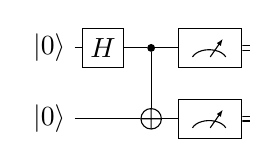
\begin{tikzpicture}[scale=1.0]
   \begin{yquant*}[register/minimum height=0.8cm]
   qubit {$\ket0$} x;
   qubit {$\ket0$} y;
   box {$H$} x;
   cnot y | x;
   measure x;
   measure y;
  \end{yquant*}
\end{tikzpicture}
\caption{\label{fig:bell}Bell circuit}
\end{subfigure}
\qquad\qquad
\begin{subfigure}[b]{.25\textwidth}
    \centering
    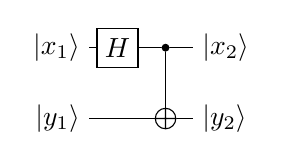
\begin{tikzpicture}[scale=1.0]
   \begin{yquant*}[register/minimum height=0.8cm]
   qubit {$\ket{x_1}$} x;
   qubit {$\ket{y_1}$} y;
   box {$H$} x;
   cnot y | x;
   output {$\ket{x_2}$} x;
   output {$\ket{y_2}$} y;
  \end{yquant*}
\end{tikzpicture}
\caption{\label{fig:bellqcore}Quantum core}
\end{subfigure}
\qquad\qquad
\begin{subfigure}[b]{.25\textwidth}
    \centering
    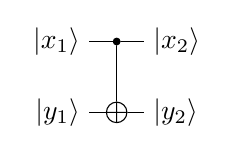
\begin{tikzpicture}[scale=1.0]
   \begin{yquant*}[register/minimum height=0.8cm]
   qubit {$\ket{x_1}$} x;
   qubit {$\ket{y_1}$} y;
   cnot y | x;
   output {$\ket{x_2}$} x;
   output {$\ket{y_2}$} y;
  \end{yquant*}
\end{tikzpicture}
\caption{\label{fig:bellccore}Classical core}
\end{subfigure}
\caption{\label{fig:bellall}A conventional quantum circuit with
  initial conditions and measurement (a); its quantum core without
  measurement and with unspecified initial and final conditions (b); and
  its classical core without explicit quantum superpositions (c).}
\end{figure}

The main ideas underlying our contributions can be illustrated with
the aid of the small examples in Fig.~\ref{fig:bellall}. In the
conventional computational mode (Fig.~\ref{fig:bell}), the execution
starts with the initial state $\ket{00}$. The first gate (Hadamard)
evolves the state to $1/\sqrt{2}~(\ket{00} + \ket{10})$ which is
transformed by the controlled-not (\cx) gate to $1/\sqrt{2}~(\ket{00} +
\ket{11})$. The measurements at the end produce 00 or 11 with equal
probability. Fig.~\ref{fig:bellqcore} keeps the quantum core of the
circuit, removing the measurements, and naming the inputs and outputs
with symbolic variables. Now, instead of setting $x_1=y_1=0$ and
computing forward as before, we can, for example, set $x_2=1$ and
$y_2=0$ and calculate backwards as follows: $\ket{10}$ evolves in the
backwards direction to $\ket{11}$ and then to
$1/\sqrt{2}~(\ket{01}-\ket{11})$. In other words, in order to observe
$x_2y_2=10$, the variable $x_1$ should be prepared in the
superposition $1/\sqrt{2}~(\ket{0}-\ket{1})$ and $y_1$ should be
prepared in the state $\ket{1}$. More interestingly, we can partially
specify the initial and final conditions. For example, we can fix
$x_1=0$ and $x_2=1$ and ask if there are any possible values for $y_1$
and $y_2$ that would be consistent with this setting. To answer the
question, we calculate, using the techniques of symbolic partial
evaluation (Methods), as follows. The initial state is $\ket{0y_1}$
which evolves to $1/\sqrt{2}~(\ket{0y_1}+\ket{1y_1})$ and then to
$1/\sqrt{2}~(\ket{0y_1}+\ket{1(1 \oplus y_1)})$ where $\oplus$ is the
exclusive-or operation and $1 \oplus y_1$ is the canonical way of
negating $y_1$ in the Algebraic Normal Form (ANF) of boolean
expressions (Methods). This final state can now be reconciled with the
specified final conditions $1y_2$ revealing that the settings are
consistent provided that $y_2 = 1 \oplus y_1$. We can, in fact, go one
step further and analyze the circuit without the Hadamard gate as
shown in Fig.~\ref{fig:bellccore}. The reasoning is that the role of
Hadamard is to introduce (modulo phase) uncertainty about whether
$x_1=0$ or $x_1=1$. But, again modulo phase, the same uncertainty can
be expressed by just using the variable $x_1$. Thus, in
Fig.~\ref{fig:bellccore}, we can set $y_1=0$ and $y_2=1$ and ask about
values of $x_1$ and $x_2$ that would be consistent with this
setting. We can calculate backwards from $\ket{x_21}$ as follows. The
state evolves to $\ket{x_2(1 \oplus x_2)}$ which can be reconciled
with the initial conditions yielding the constraints $x_1=x_2$ and $1
\oplus x_2 = 0$ whose solutions are $x_1 = x_2 = 1$.
These insights are robust and can be implemented in software (Methods)
to analyze circuits with millions of gates for the quantum algorithms
that match the template in Fig.~\ref{fig:templateQC} (including
Deutsch, Deutsch-Jozsa, Bernstein-Vazirani, Simon, Grover, and Shor's
algorithms~\cite{doi:10.1137/S0097539796300921,deutsch,deutschJozsa,365701,doi:10.1137/S0097539795293172,nielsen_chuang_2010,10.1145/237814.237866}). The
software is completely classical, performing mixed mode executions of
the classical core of the circuits, i.e., the $U_f$ block defined as
$U_f(\ket{x}\ket{y}) = \ket{x}\ket{f(x) \oplus y}$. Specifically, in
all these algorithms, the top collection of wires (which we will call
the computational register) is prepared in a uniform superposition
which can be represented using symbolic variables. The measurement of
the bottom collection of wires (which we call the ancilla register)
after barrier 2 provides partial information about the future which
is, together with the initial conditions of the ancilla register,
sufficient to symbolically execute the circuit. In each case, instead
of the conventional execution flow depicted in
Fig.~\ref{fig:templateQC}(a), we find a possible measurement outcome
$w$ at barrier (2) and perform a symbolic retrodictive execution with
a state $\ket{xw}$ going backwards to collect the constraints on $x$
that enable us to solve the problem in question.

%%%%%%%%%%%%%%%%%%%%%%%%%%%%%%%%%%%%%%%%%%%%%%%%%%%%%%%%%%%%%%%%%%%%%%%%%
\section*{Methods}

\paragraph*{Symbolic Execution of Classical Programs.}
A well-established technique to simultaneously explore multiple paths
that a classical program could take under different inputs is
\emph{symbolic
  execution}~\cite{10.1145/390016.808445,10.1145/360248.360252,howden,10.1145/800191.805647,10.1145/3182657}. In
this execution scheme, concrete values are replaced by symbols which are
initially unconstrained. As the execution proceeds, the symbols
interact with program constructs and this typically introduces
constraints on the possible values that the symbols represent. At the
end of the execution, these constraints can be solved to infer
properties of the program under consideration. 

\begin{figure}[ht]
\begin{center}
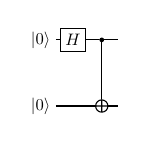
\begin{tikzpicture}[scale=0.6]
   \begin{yquant*}[register/minimum height=1.3cm]
   qubit {$\ket0$} x;
   qubit {$\ket0$} y;
   box {$H$} x;
   cnot y | x;
  \end{yquant*}
\end{tikzpicture}
\qquad
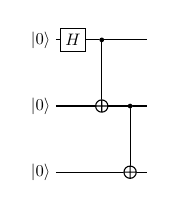
\begin{tikzpicture}[scale=0.6]
   \begin{yquant*}[register/minimum height=1.3cm]
   qubit {$\ket0$} x;
   qubit {$\ket0$} y;
   qubit {$\ket0$} z;
   box {$H$} x;
   cnot y | x;
   cnot z | y;
  \end{yquant*}
\end{tikzpicture}
\end{center}
\caption{\label{fig:bell2}Bell and GHZ States}
\end{figure}
\paragraph*{Entanglement.}
A symbolic variable represents a boolean value that can be 0 or 1;
this is similar to a qubit in a superposition $1/\sqrt{2}~ (\ket{0}
\pm \ket{1})$. Thus, it appears that $H\ket{0}$ could be represented
by a symbol~$x$ to denote the uncertainty. Surprisingly, this idea
scales to even represent maximally entangled
states. Fig.~\ref{fig:bell2} (left) shows a circuit to generate the Bell
state $1/\sqrt{2}~ (\ket{00} + \ket{11})$. By using the symbol $x$
for $H\ket{0}$, the input to the \cx-gate is $\ket{x0}$ which
evolves to $\ket{xx}$. By sharing the same symbol in two positions,
the symbolic state accurately represents the entangled Bell
state. Similarly, for the circuit in Fig.~\ref{fig:bell2} (right), the
state after the Hadamard gate is $\ket{x00}$ which evolves to
$\ket{xx0}$ and then to $\ket{xxx}$ again accurately capturing the
entanglement correlations.

Given a maximally entangled state defined with respect to a particular
tensor product decomposition, the same state may become unentangled in
a different tensor product decomposition. Given the state:
\[
 \ket{\Psi} =\ket{0}+\ket{3}+\ket{6}+\ket{9}+\ket{12}+\ket{15},
\]
one can find a 4-qubit representation (${\mathcal H}=\bigotimes_{i=1}^4
\mathbb{C}^2$)
\[
 \ket{\Psi} = \ket{0000}+\ket{0011}+\ket{0110} 
  + \ket{1001}+\ket{1100}+\ket{1111},
\]
where we used the following map $\ket{m}=\sum_{i=0}^3 x_i 2^i$, with
$m \in \mathbb{Z}$ and $x_i=0,1$.  One can use the purity~\cite{GE2004}
\[
 P_{\ket{\Psi} }=\frac{1}{4}\sum_{i=1}^4\sum_{\mu=x,y,z}\langle \Psi |
 \sigma^\mu_i \ket{\Psi}^2
\]
and confirm that the state $\ket{\Psi}$ is maximally entangled, i.e.,
has $P_{\ket{\Psi}} =0$. In contrast, in a qutrit basis (${\mathcal
  H}=\bigotimes_{i=1}^4 \mathbb{C}^3$), given the map
$\ket{m}=\sum_{i=0}^3 x_i 3^i$, with $x_i=0,1,2$, the state
\begin{eqnarray}
 \ket{\Psi} &=&\ket{0000}+\ket{0010}+\ket{0020} 
  + \ket{0100}+\ket{0110}+\ket{0120} \nonumber \\
 &=&\ket{0}\otimes(\ket{0}+\ket{1})\otimes(\ket{0}+\ket{1}+\ket{2})\otimes\ket{0}, \nonumber
\end{eqnarray}
is a product (unentangled) state. 

\begin{figure}[ht]
\begin{center}
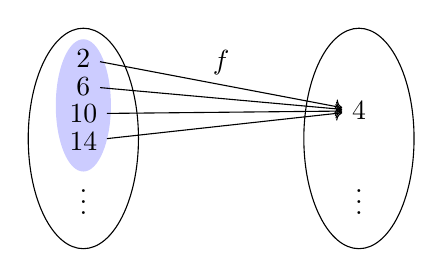
\begin{tikzpicture}[scale=0.7]
\draw (0,0) ellipse (1cm and 2cm);
\draw (5,0) circle (1cm and 2cm);
\fill[blue!20!white] (0,0.6) ellipse (0.5cm and 1.2cm);
\node (a) at (0,1.45) {2};
\node (b) at (0,0.95) {6};
\node (c) at (0,0.45) {10};
\node (d) at (0,-0.05) {14};
\node (t) at (5,0.5) {4};
\node at (0,-1) {$\vdots$};
\node at (5,-1) {$\vdots$};
\draw[->] (a) to node [above] {$f$} (t);
\draw[->] (b) -- (t);
\draw[->] (c) -- (t);
\draw[->] (d) -- (t);
\end{tikzpicture}
\end{center}
\caption{\label{fig:preimage}The pre-image of 4 under $f(x) = 7^x \mod 15$.}
\end{figure}
\paragraph*{Complexity Analysis.}
Given finite sets $A$ and $B$, a function $f : A \rightarrow B$ and an
element $y \in B$, we define $\preim{f}{y}$, the pre-image of~$y$
under~$f$, as the set $\{ x \in A ~|~ f(x) = y \}$. For example, let
$A = B = \finset{2^4}$ and let $f(x) = 7^x \mod 15$, then the
collection of values that $f$ maps to~4, $\preim{f}{4}$, is the set
$\{ 2, 6, 10, 14 \}$ as shown in Fig.~\ref{fig:preimage}. Symbolic
retrodictive execution can be seen as a method to generate boolean
formulae that describe the pre-image of the function $f$ under
study. For the example in Fig.~\ref{fig:preimage}, retrodictive
execution might generate the formulae $x_1=1$ and $x_0=0$. The
(trivial in this case) solution for the formulae is indeed the set $\{
2, 6, 10, 14 \}$. The critical points to note, however, are that: (i)
solving the equations describing the pre-image is in general an
intractable (even for quantum computers) $\mathit{NP}$-complete
problem, and (ii) solving the equations is not needed for typical
quantum algorithms. \emph{Only some global properties of the pre-image
  are needed!} Indeed, we have already seen that for solving the
Deutsch-Jozsa problem, the only thing needed was whether the formula
contains some variables. For the Bernstein-Vazirani problem, the only
thing needed was the indices of the variables occurring in the
formula. For Grover's algorithm, we only need to extract the singleton
element in the pre-image and for Shor's algorithm we ``only'' need to
extract the periodicity of the elements in the pre-image.

To appreciate the difficulty of computing pre-images in general, note
that finding the pre-image of a function subsumes several challenging
computational problems such as pre-image attacks on hash
functions~\cite{10.1007/978-3-540-25937-4_24}, predicting
environmental conditions that allow certain reactions to take place in
computational biology~\cite{Klotz2013,akutsu2009analyses}, and finding
the pre-image of feature vectors in the space induced by a kernel in
neural networks~\cite{1353287}. More to the point, the boolean
satisfiability problem SAT is expressible as a boolean function over
the input variables and solving a SAT problem is asking for the
pre-image of \textsf{true}. Indeed, based on the conjectured existence
of one-way functions which itself implies $\mathit{P} \neq
\mathit{NP}$, all these pre-images calculations are believed to be
computationally intractable in their most general setting.

The bottleneck in retrodictive execution, as we presented it, is
therefore in the symbolic execution of circuits in the ANF domain. Not
only does the execution scale with the number of gates in the circuit
but also with the size of the intermediate ANF formulae, which could
become exponential in the number of variables.

\paragraph*{Software.}
The entire suite of programs including synthesis of reversible
circuits, standard evaluation, retrodictive evaluation under various
modes, testing, debugging, and alternative representations off ANF
formulae is only ~1,500 lines of Haskell. The heart of the
implementation is this simple function:

\begin{minted}{haskell}
peG :: Value v => GToffoli s v -> ST s ()
peG (GToffoli bs cs t) = do
  controls <- mapM readSTRef cs
  tv <- readSTRef t
  let funs = map (\b -> if b then id else snot) bs
  let r = sxor tv (foldr sand one (zipWith ($) funs controls))
  writeSTRef t r
\end{minted}
The function performs symbolic evaluation of one generalized Toffoli
gates, reading the current ANF formulae for each control and producing
an appropriate ANF formula for the target.

\paragraph*{Supplementary Information.} 
\label{par:shor21}

The equations generated by retrodictive execution of the optimized
circuit for $4^x \mod{21}$ starting from observed result 1 and unknown
$x$ are:

\bigskip

$1 \oplus x_0 \oplus x_1 \oplus x_2 \oplus x_0x_2 \oplus x_0x_1x_2
\oplus x_3 \oplus x_1x_3 \oplus x_0x_1x_3 \oplus x_0x_2x_3 \oplus
x_1x_2x_3 \oplus x_4 \oplus x_0x_4 \oplus x_0x_1x_4 \oplus x_2x_4
\oplus x_1x_2x_4 \oplus x_0x_1x_2x_4 \oplus x_0x_3x_4 \oplus x_1x_3x_4
\oplus x_2x_3x_4 \oplus x_0x_2x_3x_4 \oplus x_0x_1x_2x_3x_4 \oplus x_5
\oplus x_1x_5 \oplus x_0x_1x_5 \oplus x_0x_2x_5 \oplus x_1x_2x_5
\oplus x_3x_5 \oplus x_0x_3x_5 \oplus x_0x_1x_3x_5 \oplus x_2x_3x_5
\oplus x_1x_2x_3x_5 \oplus x_0x_1x_2x_3x_5 \oplus x_0x_4x_5 \oplus
x_1x_4x_5 \oplus x_2x_4x_5 \oplus x_0x_2x_4x_5 \oplus x_0x_1x_2x_4x_5
\oplus x_3x_4x_5 \oplus x_1x_3x_4x_5 \oplus x_0x_1x_3x_4x_5 \oplus
x_0x_2x_3x_4x_5 \oplus x_1x_2x_3x_4x_5 = 1$

\bigskip

$x_1 \oplus x_0x_1 \oplus x_0x_2 \oplus x_1x_2 \oplus x_3 \oplus
x_0x_3 \oplus x_0x_1x_3 \oplus x_2x_3 \oplus x_1x_2x_3 \oplus
x_0x_1x_2x_3 \oplus x_0x_4 \oplus x_1x_4 \oplus x_2x_4 \oplus
x_0x_2x_4 \oplus x_0x_1x_2x_4 \oplus x_3x_4 \oplus x_1x_3x_4 \oplus
x_0x_1x_3x_4 \oplus x_0x_2x_3x_4 \oplus x_1x_2x_3x_4 \oplus x_5 \oplus
x_0x_5 \oplus x_0x_1x_5 \oplus x_2x_5 \oplus x_1x_2x_5 \oplus
x_0x_1x_2x_5 \oplus x_0x_3x_5 \oplus x_1x_3x_5 \oplus x_2x_3x_5 \oplus
x_0x_2x_3x_5 \oplus x_0x_1x_2x_3x_5 \oplus x_4x_5 \oplus x_1x_4x_5
\oplus x_0x_1x_4x_5 \oplus x_0x_2x_4x_5 \oplus x_1x_2x_4x_5 \oplus
x_3x_4x_5 \oplus x_0x_3x_4x_5 \oplus x_0x_1x_3x_4x_5 \oplus
x_2x_3x_4x_5 \oplus x_1x_2x_3x_4x_5 \oplus x_0x_1x_2x_3x_4x_5 = 0$

\bigskip

$x_0 \oplus x_0x_1 \oplus x_2 \oplus x_1x_2 \oplus x_0x_1x_2 \oplus
x_0x_3 \oplus x_1x_3 \oplus x_2x_3 \oplus x_0x_2x_3 \oplus
x_0x_1x_2x_3 \oplus x_4 \oplus x_1x_4 \oplus x_0x_1x_4 \oplus
x_0x_2x_4 \oplus x_1x_2x_4 \oplus x_3x_4 \oplus x_0x_3x_4 \oplus
x_0x_1x_3x_4 \oplus x_2x_3x_4 \oplus x_1x_2x_3x_4 \oplus
x_0x_1x_2x_3x_4 \oplus x_0x_5 \oplus x_1x_5 \oplus x_2x_5 \oplus
x_0x_2x_5 \oplus x_0x_1x_2x_5 \oplus x_3x_5 \oplus x_1x_3x_5 \oplus
x_0x_1x_3x_5 \oplus x_0x_2x_3x_5 \oplus x_1x_2x_3x_5 \oplus x_4x_5
\oplus x_0x_4x_5 \oplus x_0x_1x_4x_5 \oplus x_2x_4x_5 \oplus
x_1x_2x_4x_5 \oplus x_0x_1x_2x_4x_5 \oplus x_0x_3x_4x_5 \oplus
x_1x_3x_4x_5 \oplus x_2x_3x_4x_5 \oplus x_0x_2x_3x_4x_5 \oplus
x_0x_1x_2x_3x_4x_5 = 0$

\bigskip

The equations generated by retrodictive execution of the unoptimized
$4^x \mod{21}$ starting from observed result 1 and unknown $x$. The
circuit consists of 36,400 \cx-gates, 38,200 \ccx-gates, and 4,000
\cccx-gates. There are only three equations but each equation is
exponentially large.
\end{comment}

%%%%%%%%%%%%%%%%%%%%%%%%%%%%%%%%%%%%%%%%%%%%%%%%%%%%%%%%%%%%%%%%%%%%%%%%%

\bibliography{cites.bib}
\end{document}

